\chapter{Contexte et présentation}
	\section{Présentation du contexte}
	%TODO Parler du client et de son métier + besoin (cf : Cahier des charges.pdf)

	\section{Choix techno}

		%TODO Disclamer : Pas tuto SpringBoot, gradle, ionic, ... (mettre des liens tutos)

		\subsection{MySql}
		%TODO Pourquoi avoir choisi MySql et pas autre chose

		\subsection{Spring Boot}
		%TODO Pourquoi Spring boot, parler des ""parts du marchés"", avantages, ...

		\subsection{Ionic}
		%TODO Pourquoi Ionic, écrire du code en code Js, multiplateforme, ...

		\subsection{Gradle}
			%On fait une description brève car on en reparle plus en détail dans "Intéraction entre les différentes parties du projet"
			Gradle est un "build automation system" (moteur de production). Il est un équivalent plus récent et complet à Maven. Il possède de meilleure performances, possède un bon support dans de nombreux IDE et permet d'utiliser de nombreux dépots, dont ceux de Maven.

	\section{Organisation du projet}
		\subsection{Git et branches}
			\subsubsection{Branches}
			%TODO Parler de master (=version prod), develop, features/XXX

			\subsubsection{Nommenclature}
			%TODO Parler des nommenclatures (cf : fichier CONVENTIONS.md)

		\subsection{Les différents dossiers}
			\subsubsection{Doc}
			%TODO ((Parler de pk latex?))

			\subsubsection{SQL}
			%TODO Expliquer + nommenclature et table de version

			\subsubsection{Sources}
			%TODO Ionic = ionic, spring = code spring boot(webapp, rest, core) (on en reparlera plus tard dans la doc)

		\subsection{Trello}
		%TODO Fournir le lien et expliquer étiquettes, Listes

	\section{Interactions entre les différentes parties du projet}
		\subsection{Les différentes parties}
			Le projet Équida est composé de 2 applications. Une l'application web, qui est également l'application principale, une application mobile qui est à usage principal des utilisateurs. Les 2 applications s'appuient sur la même \bdd{}. L'application web y est directement connectée. L'application mobile, elle, passe par une API. En effet, si celle ci se connecterait directement à la \bdd{} comme c'est le cas pour l'application web, une personne mal intentionnée serait en mesure de décompiler l'application mobile afin d'obtenir les identifiants de la \bdd{}. L'utilisation de cette API empêche donc notamment ce problème de sécurité.

			\begin{figure}[H]
				\centering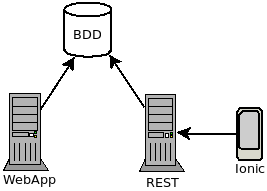
\includegraphics[width=0.45\textwidth, keepaspectratio]{res/diag_infra.png}
				\caption{La connexion à la BDD selon le projet}
			\end{figure}

			L'API ainsi que l'application web utilisent sur le Framework Spring Boot. Ces 2 applications font donc parti de 2 projets différents, "webapp" pour la partie web et "rest" pour l'api. Celles si demandant un code identique pour les Services, les Entités ainsi que les Repository, le choix a donc été fait de faire un projet commun dénomé "core" dans lequel on peut retrouver tout le code qui sera commun aux 2 autres parties, non seulement concernant les éléments cités plus haut mais également concernant les exceptions ou certains outils.

			\begin{figure}[H]
				\centering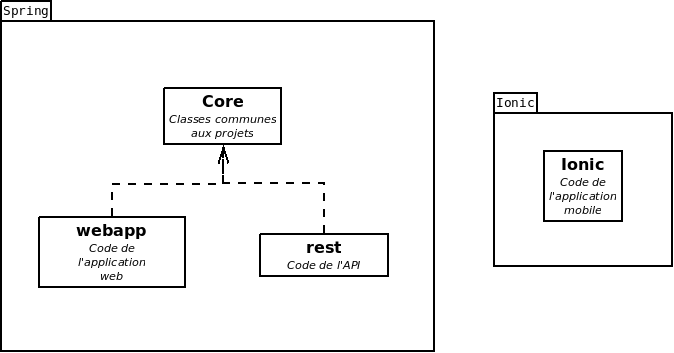
\includegraphics[width=0.75\textwidth, keepaspectratio]{res/diag_projet.png}
				\caption{Les dépendances entre les projets}
			\end{figure}

		\subsection{Configuration Gradle}

			Pour gérer correctement les différents projets basés sur Spring, leur dépendances ainsi que leur configuration nous avons donc utilisé Gradle comme mentionné plus haut. Dans le dossier "src/Spring" on retrouve le "build.gradle" qui se charge de configurer tout le projet. On peut observer la configuration suivante pour tout les projets.

			\begin{figure}[H]
				\centering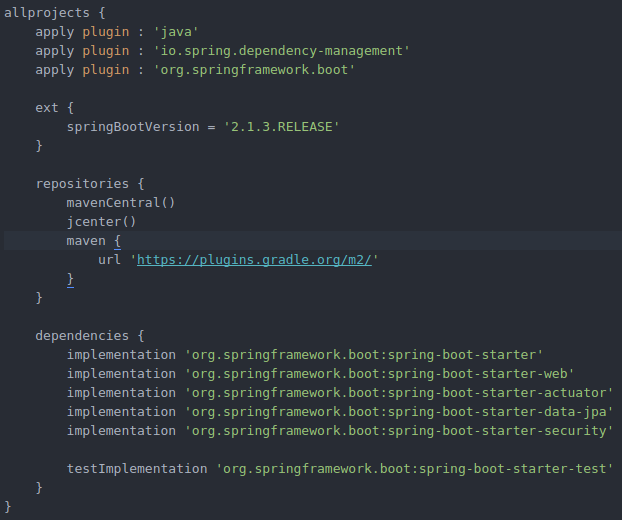
\includegraphics[width=0.75\textwidth, keepaspectratio]{res/gradle_allprojects.png}
				\caption{Configuration Gradle de tous les projets}
			\end{figure}

			On définit donc la version de Spring à utiliser, en plus des dépendences commune à chaque projet (spring-boot-starter-web, spring-boot-starter-data-jpa, ...). On va par la suite définir les dépendances uniques à chaque projet.

			\begin{figure}[H]
				\centering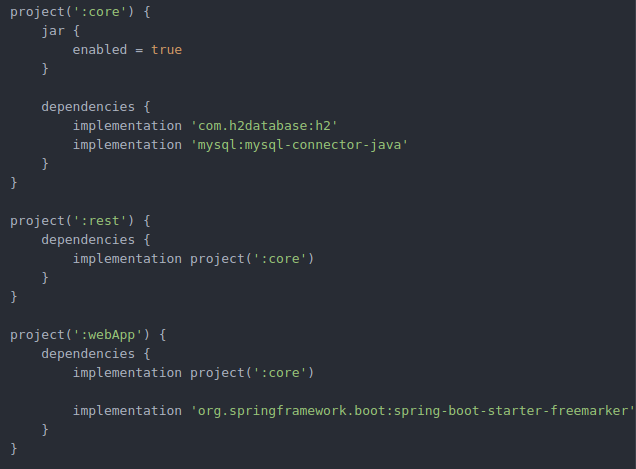
\includegraphics[width=0.75\textwidth, keepaspectratio]{res/gradle_project.png}
				\caption{Configuration Gradle individuelle des projets}
			\end{figure}

			De même, concernant le projet core, on active uniquement la compilation en jar (comme une lib) et non pas en jar bootable (comme c'est le cas lorsque l'on utilise Spring Boot).

			D'autre scripts "build.gradle" se trouvent dans chaque dossiers du projet, cependant, ceux ci ne configurent que le nom du projet à l'issue du build, la version du JDK utilisée ainsi que le package de base du projet.
